%%%%%%%%%%%%%%%%%%%%%%%%%%%%%%%%%%%%%%%%
% Masters/Doctoral Thesis 
% LaTeX Template
% Version 2.5 (27/8/17)
%
% This template was downloaded from:
% http://www.LaTeXTemplates.com
%
% Version 2.x major modifications by:
% Vel (vel@latextemplates.com)
%
% This template is based on a template by:
% Steve Gunn (http://users.ecs.soton.ac.uk/srg/softwaretools/document/templates/)
% Sunil Patel (http://www.sunilpatel.co.uk/thesis-template/)
%
% Template license:
% CC BY-NC-SA 3.0 (http://creativecommons.org/licenses/by-nc-sa/3.0/)
%
%%%%%%%%%%%%%%%%%%%%%%%%%%%%%%%%%%%%%%%%%

%----------------------------------------------------------------------------------------
%	PACKAGES AND OTHER DOCUMENT CONFIGURATIONS
%----------------------------------------------------------------------------------------

\documentclass[
11pt, % The default document font size, options: 10pt, 11pt, 12pt
oneside, % Two side (alternating margins) for binding by default, uncomment to switch to one side
spanish, % ngerman for German
singlespacing, % Single line spacing, alternatives: onehalfspacing or doublespacing
%draft, % Uncomment to enable draft mode (no pictures, no links, overfull hboxes indicated)
%nolistspacing, % If the document is onehalfspacing or doublespacing, uncomment this to set spacing in lists to single
%liststotoc, % Uncomment to add the list of figures/tables/eta, haberc to the table of contents
%toctotoc, % Uncomment to add the main table of contents to the table of contents
parskip, % Uncomment to add space between paragraphs
%nohyperref, % Uncomment to not load the hyperref package
headsepline, % Uncomment to get a line under the header
%chapterinoneline, % Uncomment to place the chapter title next to the number on one line
%consistentlayout, % Uncomment to change the layout of the declaration, abstract and acknowledgements pages to match the default layout
table
]{MastersDoctoralThesis} % The class file specifying the document structure


\usepackage{xcolor}

\usepackage{soul}
\usepackage{graphicx}
%\usepackage{subfig}


\usepackage[bottom]{footmisc}

\usepackage[utf8]{inputenc} % Required for inputting international characters
%\usepackage[T1]{fontenc} % Output font encoding for international characters

\usepackage{mathpazo} % Use the Palatino font by default
\usepackage{amsmath}
\usepackage{caption}

\usepackage{float}

\usepackage{hyperref}
\usepackage{apacite} %EN CASO DE NO USAR APA STYLE COMENTAR ESTA LINEA Y CAMBIAR EL ESTILO DE ABAJO

% \usepackage{subcaption}

%\usepackage[backend=bibtex, natbib=true]{biblatex} % Use the bibtex backend with the authoryear citation style (which resembles APA)
% SI AGREGO STYLE=AUTHORYEAR PARA QUE SEA ESTILO APA, SE ME DESORDENA EL FORMATO DE LOS AUTORES EN LA BIBLIOGRAFIA... MUY RARO, NO ENCUENTRO SOLUCION EN GOOGLE HASTA EL MOMENTO
%\usepackage[
%backend=biber,
%style=alphabetic,
%citestyle=authoryear
%]{biblatex}

% Use the bibtex backend with the authoryear citation style (which resembles APA)
%,style=authoryear,natbib=true

% \addbibresource{citas.bib} % The filename of the bibliography
\usepackage[autostyle=true]{csquotes} % Required to generate language-dependent quotes in the bibliography
\usepackage{color}
%----------------------------------------------------------------------------------------
%	MARGIN SETTINGS
%----------------------------------------------------------------------------------------

\geometry{
	paper=a4paper, % Change to letterpaper for US letter
	inner=2.5cm, % Inner margin
	outer=3.8cm, % Outer margin
	bindingoffset=.5cm, % Binding offset
	top=1.5cm, % Top margin
	bottom=1.5cm, % Bottom margin
	%showframe, % Uncomment to show how the type block is set on the page
}

%----------------------------------------------------------------------------------------
%	THESIS INFORMATION
%----------------------------------------------------------------------------------------

\thesistitle{Metodología de generación de \enquote{super-categorías} con modelos de lenguaje grande (LLM) para la mitigación del problema del \enquote{cold-start} en sistemas de recomendación.} % Your thesis title, this is used in the title and abstract, print it elsewhere with \ttitle
\thesistitleEnglish{Methodology for generating \enquote{super-categories} with large language models (LLM) to mitigate the \enquote{cold-start} problem in recommendation systems.} % Your thesis title, this is used in the title and abstract, print it elsewhere with \ttitleEnglish
\supervisor{Claudio Esteban Díaz Cifuentes\\EN CASO DE CO-GUIA} % Your supervisor's name, this is used in the title page, print it elsewhere with \supname
\examiner{NOMBRE COMISON\\2DO NOMBRE COMISION} % Your examiner's name, this is not currently used anywhere in the template, print it elsewhere with \examname
% \degree{comente esta línea y descomente la linea de degree correspondiente}
% \degree{Magíster en Ciencias de la Ingeniería, mención ESCRIBIR EL NOMBRE DE LA MENCION} % Your degree name, this is used in the title page and abstract, print it elsewhere with \degreename
% \degree{Magíster en Ingeniería Industrial e Investiagación de Operaciones} % Your degree name, this is used in the title page and abstract, print it elsewhere with \degreename
\degree{Master of Science in Data Science; Ingeniería Civil Informática} % Your degree name, this is used in the title page and abstract, print it elsewhere with \degreename
% \degreeEnglish{comment this line and choose the right degree}
% \degreeEnglish{Master of Science in Engineering, concentration XXXX}
\degreeEnglish{Master of Science in Data Science}
% \degreeEnglish{Master in Industrial Engineering and Operations Research}
\author{Fernando Andrés Zamora Carrasco} % Your name, this is used in the title page and abstract, print it elsewhere with \authorname
\addresses{} % Your address, this is not currently used anywhere in the template, print it elsewhere with \addressname
\subject{Machine Learning} % Your subject area, this is not currently used anywhere in the template, print it elsewhere with \subjectname
\keywords{machine learning, marketing, sistemas de recomendación} % Keywords for your thesis, this is not currently used anywhere in the template, print it elsewhere with \keywordnames
\university{\href{https://www.uai.cl/}{Universidad Adolfo Ibañez}} % Your university's name and URL, this is used in the title page and abstract, print it elsewhere with \univname
\department{\href{https://ingenieria.uai.cl/}{Departamento de Ciencias de Datos}} % Your department's name and URL, this is used in the title page and abstract, print it elsewhere with \deptname
\faculty{\href{https://ingenieria.uai.cl/}{Facultad de Ingeniería y Ciencias}} % Your faculty's name and URL, this is used in the title page and abstract, print it elsewhere with \facname
\facultyEnglish{\href{https://ingenieria.uai.cl/}{Faculty of Engineering and Science}} % Your faculty's name and URL, this is used in the title page and abstract, print it elsewhere with \facname

\AtBeginDocument{
\hypersetup{pdftitle=\ttitle} % Set the PDF's title to your title
\hypersetup{pdfauthor=\authorname} % Set the PDF's author to your name
\hypersetup{pdfkeywords=\keywordnames} % Set the PDF's keywords to your keywords
}

\begin{document}

\frontmatter % Use roman page numbering style (i, ii, iii, iv...) for the pre-content pages

\pagestyle{plain} % Default to the plain heading style until the thesis style is called for the body content

%----------------------------------------------------------------------------------------
%	TITLE PAGE
%----------------------------------------------------------------------------------------

\begin{titlepage}
\begin{center}

\vspace*{.06\textheight}
{\scshape\LARGE \univname\par}\vspace{1.5cm} % University name
\textsc{\Large Tesis de Magíster}\\[0.5cm] % Thesis type

\HRule \\[0.4cm] % Horizontal line
{\LARGE \bfseries \ttitle\par}\vspace{0.4cm} % Thesis title
\HRule \\[1.5cm] % Horizontal line
 
\begin{minipage}[t]{0.4\textwidth}
\begin{flushleft} \large
\emph{Autor:}\\
{\authorname} % Author name - remove the \href bracket to remove the link
\end{flushleft}
\end{minipage}
\begin{minipage}[t]{0.4\textwidth}
\begin{flushright} \large
\emph{Profesores guía:} \\
\supname\\
\vspace{5mm}
\emph{Comité de defensa:} \\
\examname\\
%\href{https://ingenieria.uai.cl/profesor/paginaWeb1/}{\supname} \\% Supervisor name - remove the \href bracket to remove the link  
%\href{https://ingenieria.uai.cl/profesor/paginaWeb2/}{\examname} % Supervisor name - remove the \href bracket to remove the link  
\end{flushright}
\end{minipage}\\[2.5cm]
 
\vfill

\large \textit{Tesis realizada acorde a los requerimientos para la obtención de los grados/títulos de\\ \textbf{\degreename}}\\[0.3cm] % University requirement text
\textit{de la}\\[0.4cm]
\facname\\[1.5cm] % Research group name and department name
 
\vfill

{\large \today}\\[2cm] % Date

\includegraphics[width=5cm]{fic.png} % University/department logo - uncomment to place it
 
\vfill
\end{center}
\end{titlepage}

%----------------------------------------------------------------------------------------
%	ABSTRACT PAGE
%----------------------------------------------------------------------------------------

\begin{resumen}
\addchaptertocentry{\abstractname} % Add the abstract to the table of contents

Resuma en no más de 1 página el contenido de su propuesta. Como idea general, debería tener un párrafo por cada uno de los puntos (capítulos) que cubre el trabajo.

Sed ullamcorper quam eu nisl interdum at interdum enim egestas. Aliquam placerat justo sed lectus lobortis ut porta nisl porttitor. Vestibulum mi dolor, lacinia molestie gravida at, tempus vitae ligula. Donec eget quam sapien, in viverra eros. Donec pellentesque justo a massa fringilla non vestibulum metus vestibulum. Vestibulum in orci quis felis tempor lacinia. Vivamus ornare ultrices facilisis. Ut hendrerit volutpat vulputate. Morbi condimentum venenatis augue, id porta ipsum vulputate in. Curabitur luctus tempus justo. Vestibulum risus lectus, adipiscing nec condimentum quis, condimentum nec nisl. Aliquam dictum sagittis velit sed iaculis. Morbi tristique augue sit amet nulla pulvinar id facilisis ligula mollis. Nam elit libero, tincidunt ut aliquam at, molestie in quam. Aenean rhoncus vehicula hendrerit.

Sed ullamcorper quam eu nisl interdum at interdum enim egestas. Aliquam placerat justo sed lectus lobortis ut porta nisl porttitor. Vestibulum mi dolor, lacinia molestie gravida at, tempus vitae ligula. Donec eget quam sapien, in viverra eros. Donec pellentesque justo a massa fringilla non vestibulum metus vestibulum. Vestibulum in orci quis felis tempor lacinia. Vivamus ornare ultrices facilisis. Ut hendrerit volutpat vulputate. Morbi condimentum venenatis augue, id porta ipsum vulputate in. Curabitur luctus tempus justo. Vestibulum risus lectus, adipiscing nec condimentum quis, condimentum nec nisl. Aliquam dictum sagittis velit sed iaculis. Morbi tristique augue sit amet nulla pulvinar id facilisis ligula mollis. Nam elit libero, tincidunt ut aliquam at, molestie in quam. Aenean rhoncus vehicula hendrerit.

\textbf{Palabras clave:} LISTADO DE PALABRAS SEPARADAS POR ,.
\end{resumen}

\begin{abstract}
\addchaptertocentry{Abstract} % Add the abstract to the table of contents

IN ENGLISH

\textbf{Keywords:} ENGLISH KEYWORDS.

\end{abstract}

%----------------------------------------------------------------------------------------
%	ACKNOWLEDGEMENTS
%----------------------------------------------------------------------------------------

%\begin{acknowledgements}
%\addchaptertocentry{\acknowledgementname} % Add the acknowledgements to the table of contents
%The acknreturnowledgments and the people to thank go here, don't forget to include your project advisor\ldots
%\end{acknowledgements}

%----------------------------------------------------------------------------------------
%	LIST OF CONTENTS/FIGURES/TABLES PAGES
%----------------------------------------------------------------------------------------

\tableofcontents % Prints the main table of contents

%\listoffigures % Prints the list of figures

%\listoftables % Prints the list of tables

%----------------------------------------------------------------------------------------
%	ABBREVIATIONS
%----------------------------------------------------------------------------------------

%\begin{abbreviations}{ll} % Include a list of abbreviations (a table of two columns)

%\textbf{ACHS} & \textbf{A}sociación \textbf{C}hilena \textbf{D}e \textbf{S}eguridad\\
%\textbf{SUSESO} & \textbf{S}uperintendencia \textbf{D}e \textbf{S}eguridad \textbf{S}ocial\\
%\textbf{MUSEG} & \textbf{M}utual \textbf{D}e \textbf{S}eguridad \textbf{D}e \textbf{L}a \textbf{C}ámara \textbf{C}hilena \textbf{D}e \textbf{L}a  \textbf{C}onstrucción \\

%\end{abbreviations}

%----------------------------------------------------------------------------------------
%	THESIS CONTENT - CHAPTERS
%----------------------------------------------------------------------------------------

\mainmatter % Begin numeric (1,2,3...) page numbering

\pagestyle{thesis} % Return the page headers back to the "thesis" style

% Include the chapters of the thesis as separate files from the Chapters folder
% Uncomment the lines as you write the chapters

% Chapter 1
\chapter{Introducción} % Main chapter title
\label{sec:Introduccion} % For referencing the chapter elsewhere, use

\textbf{OMITIR ESTA SECCION PARA EL CASO DEL MAGISTER EN CIENCIAS DE LA INGENIER\'IA}

De forma de acotar la propuesta lo máximo posible, este capítulo debería responder contener al menos los siguientes puntos:
\begin{itemize}
\item Una breve descripción del lugar donde está generada la oportunidad.
\item El contexto u oportunidad de investigación.
\item La importancia y motivación de la investigación y cómo su trabajo es relevante.
\end{itemize}

\newpage
Los sistemas de recomendación tienen una gran importancia en la actualidad, puesto que permiten personalizar la experiencia del usuario en diversas plataformas digitales. 

Estos sistemas utilizan como entrada grandes volúmenes de datos generados por las interacciones de los usuarios con los productos o servicios ofrecidos. A través del análisis de estos datos, los sistemas de recomendación pueden identificar patrones y preferencias individuales, lo que les permite sugerir productos o servicios que se ajusten a los intereses específicos de cada usuario.

Entonces, ¿qué sucede cuando los datos son escasos o inexistentes? Este es el problema conocido como \enquote{cold start} o \enquote{arranque en frío}. En tales situaciones, los sistemas de recomendación enfrentan dificultades para generar sugerencias precisas debido a la falta de información suficiente sobre las preferencias del usuario o las características del producto.

Por lo tanto, el objetivo de esta tesis es investigar y desarrollar una metodología que permita mitigar el problema del \enquote{cold start} en sistemas de recomendación, utilizando técnicas de dominios de información interrelacionados.

Para ello, se trabajará en conjunto con la empresa Falabella Tecnología Corporativa, que cuenta con una amplia base de datos de usuarios y productos en sus plataformas de comercio electrónico, así como distintas unidades de negocio que pueden proporcionar información complementaria para abordar el problema del \enquote{cold start} \cite{L__2012} $\leftarrow$ cita de ejemplo/no tiene nada que ver con el párrafo.
% Chapter 1
\chapter{Definición del problema u oportunidad} % Main chapter title
\label{sec:problema} % For referencing the chapter elsewhere, use

Este capítulo debe contener la exposición general del problema. Con respecto al problema se debe responder las siguientes preguntas:
\begin{itemize}
	\item	¿Cuál es el problema u oportunidad abordado por el proyecto? ¿Es posible cuantificarlo?
	\item	¿Cuáles son las causas de la existencia de este problema u oportunidad? Haga referencia a publicaciones y/u otros antecedentes que validen estas causas.
	\item Explique cómo la memoria ayudará a abordar este problema.
	
\end{itemize}

\section{Ejemplos de latex}

Sed ullamcorper quam eu nisl interdum at interdum enim egestas. Aliquam placerat justo sed lectus lobortis ut porta nisl porttitor. Vestibulum mi dolor, lacinia molestie gravida at, tempus vitae ligula. Donec eget quam sapien, in viverra eros. Donec pellentesque justo a massa fringilla non vestibulum metus vestibulum. Vestibulum in orci quis felis tempor lacinia. Vivamus ornare ultrices facilisis. Ut hendrerit volutpat vulputate. Morbi condimentum venenatis augue, id porta ipsum vulputate in. Curabitur luctus tempus justo. Vestibulum risus lectus, adipiscing nec condimentum quis, condimentum nec nisl. Aliquam dictum sagittis velit sed iaculis. Morbi tristique augue sit amet nulla pulvinar id facilisis ligula mollis. Nam elit libero, tincidunt ut aliquam at, molestie in quam. Aenean rhoncus vehicula hendrerit.

\begin{figure}[th]
	\centering
	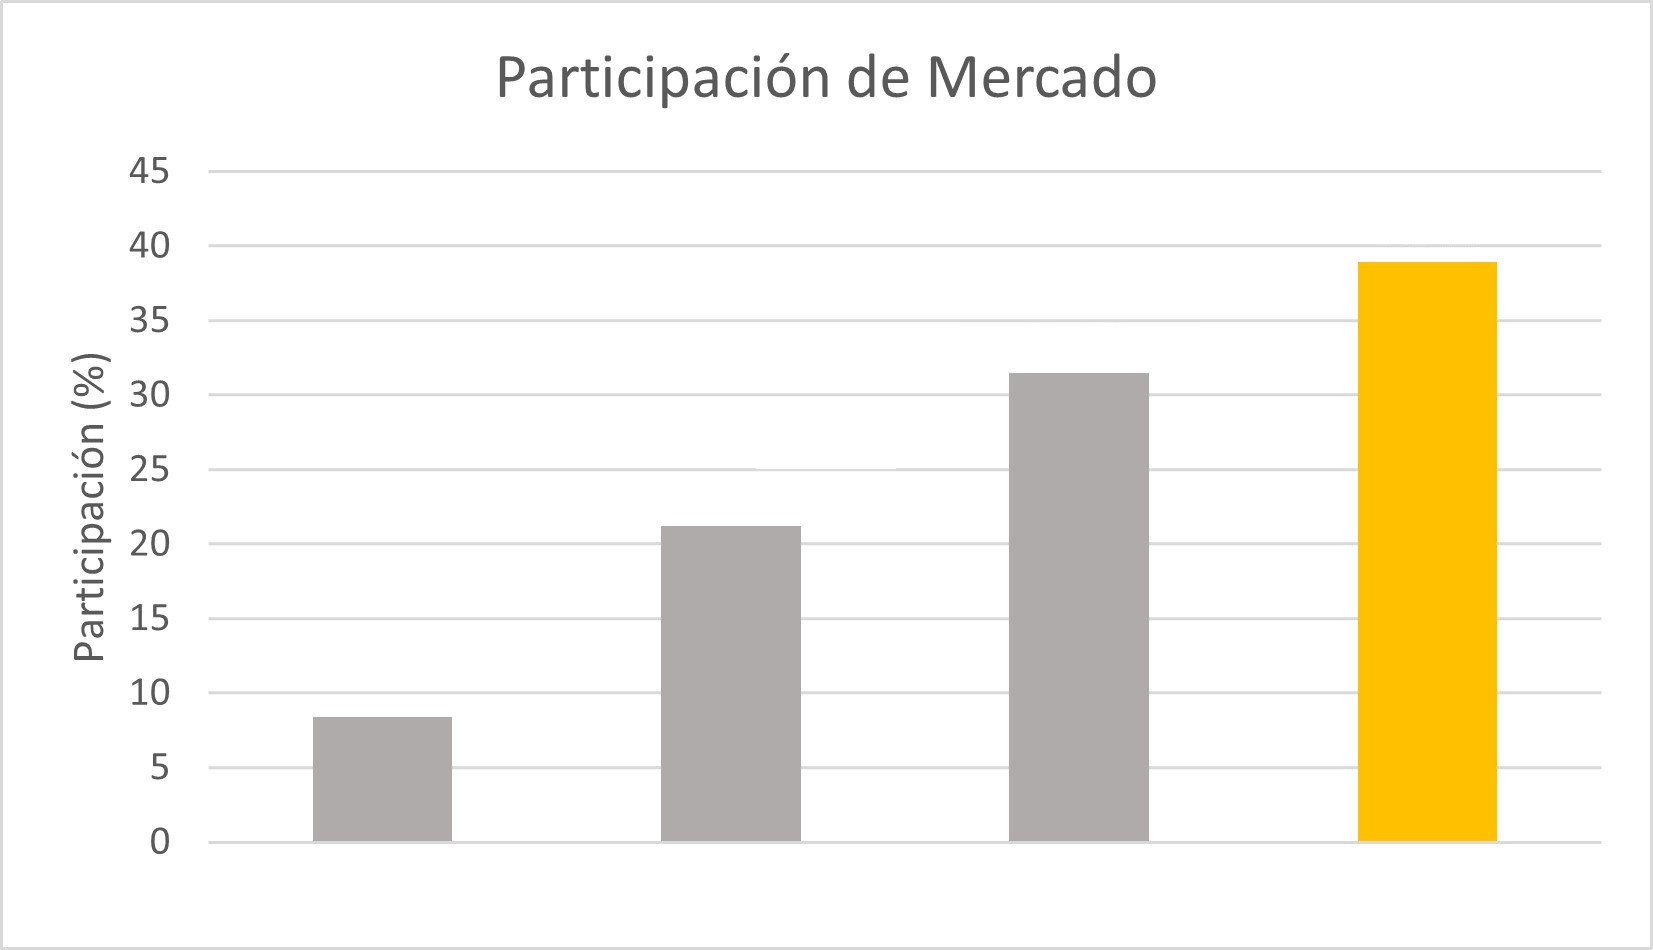
\includegraphics[width=10cm]{Figures/Ejemplo}
	\caption{Comparación de la participación de mercado entre mutuales, a enero 2020.}
	\label{fig:Ejemplo}
\end{figure}

% Citando Figura~\ref{fig:Ejemplo} de la sección~\ref{sec:problema}

Lista de items
\begin{itemize}
	\item \textbf{Componente A:} Sed ullamcorper quam eu nisl interdum at interdum enim egestas. Aliquam placerat justo sed lectus lobortis ut porta nisl porttitor. Vestibulum mi dolor, lacinia molestie gravida at, tempus vitae ligula. Donec eget quam sapien, in viverra eros. Donec pellentesque justo a massa fringilla non vestibulum metus vestibulum. Vestibulum in orci quis felis tempor lacinia. Vivamus ornare ultrices facilisis. Ut hendrerit volutpat vulputate. Morbi condimentum venenatis augue, id porta ipsum vulputate in.
	\item \textbf{Componente B:} Sed ullamcorper quam eu nisl interdum at interdum enim egestas. Aliquam placerat justo sed lectus lobortis ut porta nisl porttitor. Vestibulum mi dolor, lacinia molestie gravida at, tempus vitae ligula. Donec eget quam sapien, in viverra eros. Donec pellentesque justo a massa fringilla non vestibulum metus vestibulum. Vestibulum in orci quis felis tempor lacinia. Vivamus ornare ultrices facilisis. Ut hendrerit volutpat vulputate. Morbi condimentum venenatis augue, id porta ipsum vulputate in.
\end{itemize}

Lista enumerada
\begin{enumerate}
	\item \textbf{Componente A:} Sed ullamcorper quam eu nisl interdum at interdum enim egestas. Aliquam placerat justo sed lectus lobortis ut porta nisl porttitor. Vestibulum mi dolor, lacinia molestie gravida at, tempus vitae ligula. Donec eget quam sapien, in viverra eros. Donec pellentesque justo a massa fringilla non vestibulum metus vestibulum. Vestibulum in orci quis felis tempor lacinia. Vivamus ornare ultrices facilisis. Ut hendrerit volutpat vulputate. Morbi condimentum venenatis augue, id porta ipsum vulputate in.
	\item \textbf{Componente B:} Sed ullamcorper quam eu nisl interdum at interdum enim egestas. Aliquam placerat justo sed lectus lobortis ut porta nisl porttitor. Vestibulum mi dolor, lacinia molestie gravida at, tempus vitae ligula. Donec eget quam sapien, in viverra eros. Donec pellentesque justo a massa fringilla non vestibulum metus vestibulum. Vestibulum in orci quis felis tempor lacinia. Vivamus ornare ultrices facilisis. Ut hendrerit volutpat vulputate. Morbi condimentum venenatis augue, id porta ipsum vulputate in.
\end{enumerate}

% Citas a libro \cite{ejemploLibro} o paper~\cite{ejemploPaper}. Usted puede agregar otros tipos como journal o techincal report
\newpage

Falabella Tecnología Corporativa actualmente posee un sistema de recomendación (Implicit Collaborative Filtering - Matrix Factorization) desarrollado en BigQuery ML (BQML) que presenta varias limitaciones importantes para el negocio: es demasiado simple para abordar la complejidad del comportamiento del cliente, tiene un bajo nivel de personalización y utiliza únicamente el identificador del cliente como dato de entrada principal, desaprovechando datos relevantes como características demográficas, comportamientos históricos y segmentaciones internas.

Estas limitaciones restrigen la capacidad del sistema para generar recomendaciones personalizadas que maximicen la efectividad de las campañas de marketing. Por lo tanto, es crucial desarrollar un nuevo enfoque que integre estos datos adicionales para mejorar la precisión y relevancia de las recomendaciones, alineándolas mejor con las necesidades y preferencias individuales de los clientes. Esto permitirá optimizar las estrategias de marketing, aumentar la satisfacción del cliente y, en última instancia, mejorar los resultados comerciales de Falabella Tecnología Corporativa.

Me falta un puente para conectar lo propuesto en el archivo de la propuesta del proyecto de tesis (los párrafos anteriores) con el sistema de agentes desarrollado y lo relacionado a los Cross-Domain Recommender Systems (CDRS).

\begin{figure}[th]
	\centering
	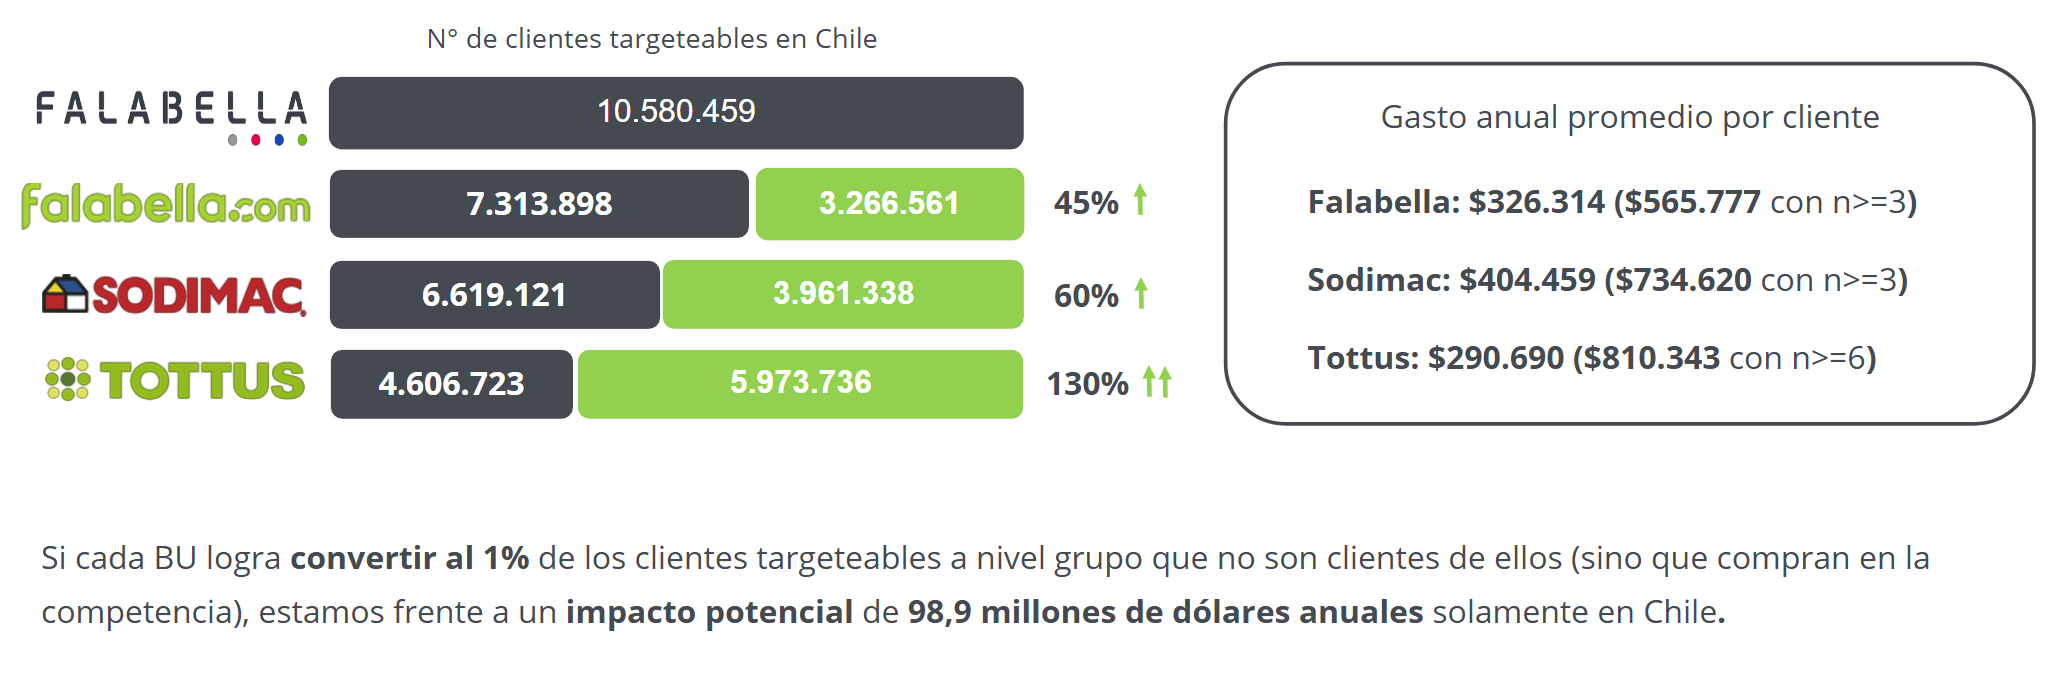
\includegraphics[width=\textwidth]{Figures/grafica Matias.png}
	\caption{Costo de oportunidad de las limitaciones del sistema de recomendación actual. Hay un par de errores menores en esta gráfica que corregiré en la versión final.}
	\label{fig:Limitaciones_Sistema_Actual}
\end{figure}

Como se puede visualizar en la figura anterior, la implementación del sistema actual está desaprovechando un mayor número de clientes potenciales, lo que se traduce en una pérdida significativa de ingresos para la empresa. Esta situación resalta la necesidad de mejorar el sistema de recomendación para captar mejor las oportunidades de venta y maximizar los beneficios comerciales. Al implementar un sistema de recomendación basado en dominios cruzados (CDRS) que utilice datos de las diferentes unidades de negocio de Falabella, se espera reducir este costo de oportunidad al aumentar la precisión y relevancia de las recomendaciones para clientes nuevos en situación de \enquote{cold-start}. Esto permitirá a la empresa aprovechar al máximo su base de clientes y mejorar su desempeño en el mercado altamente competitivo.
% Chapter 1

\chapter{Estado del arte} % Main chapter title
\label{sec:Estado Arte} % For referencing the chapter elsewhere, use

El estado del arte debería al menos responder a las siguientes preguntas:
\begin{itemize}
	\item ¿Cómo se ha enfrentado o se está enfrentando este problema u oportunidad en la literatura académica? 
	\item ¿Existen proyectos en desarrollo en la misma línea de investigación? 
	\item ¿Qué soluciones y métodos ya existen? 
\end{itemize}

Considere información nacional e internacional actualizada sobre publicaciones, proyectos tecnológicos y líneas de investigación y desarrollo en empresas u otro tipo de organizaciones. 

Dependiendo del tipo de tesis, en algunos casos se hace una búsqueda de patentes y de otros registros de propiedad intelectual, a nivel nacional e internacional, relativos al problema/oportunidad que se piensa abordar e indicar los resultados de la búsqueda. 

Realice una búsqueda y análisis de estándares, normas y reglamentaciones, tanto nacionales como extranjeras e internacionales, pertinentes y aplicables al tema del proyecto. 

Tiene 3 o 4 subsecciones. Son como 4\/6 planas. 
\begin{itemize}
	\item Sistemas de recomendación.
	\item \enquote{cold-start} problem.
	\item Atributos/features en sistemas de recomendación.
	\item Modelos de lenguaje grande en sistemas de recomendación.
\end{itemize}
\chapter{Hipótesis y objetivos} % Main chapter title
\label{sec:Hipotesis} % For referencing the chapter elsewhere, use

La tesis deberá tener hipótesis y/o objetivos (general y específicos). Discutir con su profesor guía para más detalles.
\chapter{Metodología} % Main chapter title
\label{sec:Metodologia} % For referencing the chapter elsewhere, use

Describa la metodología utilizada o por utilizar durante su proyecto, sustente debidamente, con un análisis bibliográfico de las metodologías disponibles, la elección de esta metodología por sobre otras. La idea de una metodologia, es que alguien pueda leerla y pueda replicar su trabajo, obteniendo los mismos resultados. 
\chapter{Resultados y análisis} % Main chapter title
\label{sec:resultados} % For referencing the chapter elsewhere, use

Para cada objetivo específico, describa los resultados obtenidos, analícelos y explíquelos claramente.
\chapter{Conclusiones} % Main chapter title
\label{sec:conclusiones} % For referencing the chapter elsewhere, use

Conclusiones de su trabajo: ¿se cumplieron los objetivos? ¿se validó la hipótesis? Debería además incluir líneas de investigación futura.

% Especifica el estilo de la bibliografía
\bibliographystyle{apacite} 
% \bibliographystyle{ieeetr}

% Llama a tu archivo .bib
\bibliography{citas}

%----------------------------------------------------------------------------------------
%	THESIS CONTENT - APPENDICES
%----------------------------------------------------------------------------------------

\appendix % Cue to tell LaTeX that the following "chapters" are Appendices

% Include the appendices of the thesis as separate files from the Appendices folder
% Uncomment the lines as you write the Appendices

% Appendix Template

\chapter{Título del apéndice} % Main appendix title

\label{AppendixX} % Change X to a consecutive letter; for referencing this appendix elsewhere, use \ref{AppendixX}

Write your Appendix content here.

%----------------------------------------------------------------------------------------
%	BIBLIOGRAPHY
%----------------------------------------------------------------------------------------


%\printbibliography[heading=bibintoc]
%\printbibliography

%----------------------------------------------------------------------------------------

\end{document}